% Graphic for TeX using PGF
% Title: /home/gabs48/mit/thesis/graphic/arch.dia
% Creator: Dia v0.97.2
% CreationDate: Fri Oct 10 17:15:52 2014
% For: gabs48
% \usepackage{tikz}
% The following commands are not supported in PSTricks at present
% We define them conditionally, so when they are implemented,
% this pgf file will use them.
\ifx\du\undefined
  \newlength{\du}
\fi
\setlength{\du}{15\unitlength}
\begin{tikzpicture}
\pgftransformxscale{0.600000}
\pgftransformyscale{-0.600000}
\definecolor{dialinecolor}{rgb}{0.000000, 0.000000, 0.000000}
\pgfsetstrokecolor{dialinecolor}
\definecolor{dialinecolor}{rgb}{1.000000, 1.000000, 1.000000}
\pgfsetfillcolor{dialinecolor}
\pgfsetlinewidth{0.100000\du}
\pgfsetdash{}{0pt}
{\pgfsetcornersarced{\pgfpoint{0.500000\du}{0.500000\du}}\definecolor{dialinecolor}{rgb}{0.474510, 0.741176, 0.603922}
\pgfsetfillcolor{dialinecolor}
\fill (8.393256\du,11.632739\du)--(8.393256\du,15.032739\du)--(24.693256\du,15.032739\du)--(24.693256\du,11.632739\du)--cycle;
}{\pgfsetcornersarced{\pgfpoint{0.500000\du}{0.500000\du}}\definecolor{dialinecolor}{rgb}{0.043137, 0.282353, 0.419608}
\pgfsetstrokecolor{dialinecolor}
\draw (8.393256\du,11.632739\du)--(8.393256\du,15.032739\du)--(24.693256\du,15.032739\du)--(24.693256\du,11.632739\du)--cycle;
}% setfont left to latex
\definecolor{dialinecolor}{rgb}{0.043137, 0.282353, 0.419608}
\pgfsetstrokecolor{dialinecolor}
\node at (16.543256\du,12.727739\du){- Calculate $\sigma_t^i = f(C_T^i)$};
% setfont left to latex
\definecolor{dialinecolor}{rgb}{0.043137, 0.282353, 0.419608}
\pgfsetstrokecolor{dialinecolor}
\node at (16.543256\du,13.527739\du){- Calculate $\sigma_s^i$ as the second order variance around $p_T^{i}$};
% setfont left to latex
\definecolor{dialinecolor}{rgb}{0.043137, 0.282353, 0.419608}
\pgfsetstrokecolor{dialinecolor}
\node at (16.543256\du,14.327739\du){- Calculate $\sigma_s^i = \mathsf{max}(\sigma_t^i, \sigma_s^i)$};
\definecolor{dialinecolor}{rgb}{0.658824, 0.858824, 0.658824}
\pgfsetfillcolor{dialinecolor}
\pgfpathellipse{\pgfpoint{42.058077\du}{1.812780\du}}{\pgfpoint{9.090108\du}{0\du}}{\pgfpoint{0\du}{1.527626\du}}
\pgfusepath{fill}
\pgfsetlinewidth{0.150000\du}
\pgfsetdash{}{0pt}
\pgfsetdash{}{0pt}
\definecolor{dialinecolor}{rgb}{0.043137, 0.282353, 0.419608}
\pgfsetstrokecolor{dialinecolor}
\pgfpathellipse{\pgfpoint{42.058077\du}{1.812780\du}}{\pgfpoint{9.090108\du}{0\du}}{\pgfpoint{0\du}{1.527626\du}}
\pgfusepath{stroke}
\definecolor{dialinecolor}{rgb}{0.811765, 0.941176, 0.619608}
\pgfsetfillcolor{dialinecolor}
\fill (29.385659\du,3.147960\du)--(38.634070\du,5.623995\du)--(29.385659\du,8.100030\du)--(20.137247\du,5.623995\du)--cycle;
\pgfsetlinewidth{0.150000\du}
\pgfsetdash{}{0pt}
\pgfsetdash{}{0pt}
\pgfsetmiterjoin
\definecolor{dialinecolor}{rgb}{0.043137, 0.282353, 0.419608}
\pgfsetstrokecolor{dialinecolor}
\draw (29.385659\du,3.147960\du)--(38.634070\du,5.623995\du)--(29.385659\du,8.100030\du)--(20.137247\du,5.623995\du)--cycle;
% setfont left to latex
\definecolor{dialinecolor}{rgb}{0.043137, 0.282353, 0.419608}
\pgfsetstrokecolor{dialinecolor}
\node at (29.385659\du,5.018995\du){For each $p_T^i \in D_T$, $p_T^i ?\in \mathcal{D}$};
% setfont left to latex
\definecolor{dialinecolor}{rgb}{0.043137, 0.282353, 0.419608}
\pgfsetstrokecolor{dialinecolor}
\node at (29.385659\du,5.818995\du){where $\mathcal{D} = \{p_T^i\}$ : $p_T^i$ is also framed};
% setfont left to latex
\definecolor{dialinecolor}{rgb}{0.043137, 0.282353, 0.419608}
\pgfsetstrokecolor{dialinecolor}
\node at (29.385659\du,6.618995\du){by $I_L$ and $I_R$};
\definecolor{dialinecolor}{rgb}{0.658824, 0.858824, 0.658824}
\pgfsetfillcolor{dialinecolor}
\pgfpathellipse{\pgfpoint{29.387845\du}{-0.057395\du}}{\pgfpoint{2.216383\du}{0\du}}{\pgfpoint{0\du}{0.890342\du}}
\pgfusepath{fill}
\pgfsetlinewidth{0.150000\du}
\pgfsetdash{}{0pt}
\pgfsetdash{}{0pt}
\definecolor{dialinecolor}{rgb}{0.043137, 0.282353, 0.419608}
\pgfsetstrokecolor{dialinecolor}
\pgfpathellipse{\pgfpoint{29.387845\du}{-0.057395\du}}{\pgfpoint{2.216383\du}{0\du}}{\pgfpoint{0\du}{0.890342\du}}
\pgfusepath{stroke}
\pgfsetlinewidth{0.150000\du}
\pgfsetdash{}{0pt}
\pgfsetdash{}{0pt}
\pgfsetbuttcap
\pgfsetmiterjoin
\pgfsetlinewidth{0.150000\du}
\pgfsetbuttcap
\pgfsetmiterjoin
\pgfsetdash{}{0pt}
\definecolor{dialinecolor}{rgb}{0.811765, 0.941176, 0.619608}
\pgfsetfillcolor{dialinecolor}
\pgfpathmoveto{\pgfpoint{8.503452\du}{8.203952\du}}
\pgfpathlineto{\pgfpoint{19.225442\du}{8.203952\du}}
\pgfpathlineto{\pgfpoint{17.081044\du}{6.253952\du}}
\pgfpathlineto{\pgfpoint{10.647850\du}{6.253952\du}}
\pgfpathlineto{\pgfpoint{8.503452\du}{8.203952\du}}
\pgfusepath{fill}
\definecolor{dialinecolor}{rgb}{0.043137, 0.282353, 0.419608}
\pgfsetstrokecolor{dialinecolor}
\pgfpathmoveto{\pgfpoint{8.503452\du}{8.203952\du}}
\pgfpathlineto{\pgfpoint{19.225442\du}{8.203952\du}}
\pgfpathlineto{\pgfpoint{17.081044\du}{6.253952\du}}
\pgfpathlineto{\pgfpoint{10.647850\du}{6.253952\du}}
\pgfpathlineto{\pgfpoint{8.503452\du}{8.203952\du}}
\pgfusepath{stroke}
% setfont left to latex
\definecolor{dialinecolor}{rgb}{0.043137, 0.282353, 0.419608}
\pgfsetstrokecolor{dialinecolor}
\node at (13.864447\du,7.028952\du){For each $p_i \in \mathcal{D}$};
% setfont left to latex
\definecolor{dialinecolor}{rgb}{0.043137, 0.282353, 0.419608}
\pgfsetstrokecolor{dialinecolor}
\node at (13.864447\du,7.828952\du){where $p^i = (u_T^i, v_T^i, d_T^i)$};
\pgfsetlinewidth{0.100000\du}
\pgfsetdash{}{0pt}
{\pgfsetcornersarced{\pgfpoint{0.500000\du}{0.500000\du}}\definecolor{dialinecolor}{rgb}{0.474510, 0.741176, 0.603922}
\pgfsetfillcolor{dialinecolor}
\fill (8.527961\du,17.402406\du)--(8.527961\du,20.802406\du)--(24.550461\du,20.802406\du)--(24.550461\du,17.402406\du)--cycle;
}{\pgfsetcornersarced{\pgfpoint{0.500000\du}{0.500000\du}}\definecolor{dialinecolor}{rgb}{0.043137, 0.282353, 0.419608}
\pgfsetstrokecolor{dialinecolor}
\draw (8.527961\du,17.402406\du)--(8.527961\du,20.802406\du)--(24.550461\du,20.802406\du)--(24.550461\du,17.402406\du)--cycle;
}% setfont left to latex
\definecolor{dialinecolor}{rgb}{0.043137, 0.282353, 0.419608}
\pgfsetstrokecolor{dialinecolor}
\node at (16.539211\du,18.497406\du){Create the interval $[d_T^i - 3 \sigma_w;\,d_T^i + 3 \sigma_w]$};
% setfont left to latex
\definecolor{dialinecolor}{rgb}{0.043137, 0.282353, 0.419608}
\pgfsetstrokecolor{dialinecolor}
\node at (16.539211\du,19.297406\du){divided in m steps};
% setfont left to latex
\definecolor{dialinecolor}{rgb}{0.043137, 0.282353, 0.419608}
\pgfsetstrokecolor{dialinecolor}
\node at (16.539211\du,20.097406\du){of size $\epsilon_D/k_{int}$};
\pgfsetlinewidth{0.150000\du}
\pgfsetdash{}{0pt}
\pgfsetdash{}{0pt}
\pgfsetbuttcap
\pgfsetmiterjoin
\pgfsetlinewidth{0.150000\du}
\pgfsetbuttcap
\pgfsetmiterjoin
\pgfsetdash{}{0pt}
\definecolor{dialinecolor}{rgb}{0.811765, 0.941176, 0.619608}
\pgfsetfillcolor{dialinecolor}
\pgfpathmoveto{\pgfpoint{4.471471\du}{25.824234\du}}
\pgfpathlineto{\pgfpoint{28.590841\du}{25.824234\du}}
\pgfpathlineto{\pgfpoint{23.766967\du}{23.874234\du}}
\pgfpathlineto{\pgfpoint{9.295345\du}{23.874234\du}}
\pgfpathlineto{\pgfpoint{4.471471\du}{25.824234\du}}
\pgfusepath{fill}
\definecolor{dialinecolor}{rgb}{0.043137, 0.282353, 0.419608}
\pgfsetstrokecolor{dialinecolor}
\pgfpathmoveto{\pgfpoint{4.471471\du}{25.824234\du}}
\pgfpathlineto{\pgfpoint{28.590841\du}{25.824234\du}}
\pgfpathlineto{\pgfpoint{23.766967\du}{23.874234\du}}
\pgfpathlineto{\pgfpoint{9.295345\du}{23.874234\du}}
\pgfpathlineto{\pgfpoint{4.471471\du}{25.824234\du}}
\pgfusepath{stroke}
% setfont left to latex
\definecolor{dialinecolor}{rgb}{0.043137, 0.282353, 0.419608}
\pgfsetstrokecolor{dialinecolor}
\node at (16.531156\du,24.649234\du){For each $p_T^{i,j} \in d_T^i - 3 \sigma_w;\,d_T^i + 3 \sigma_w]$};
% setfont left to latex
\definecolor{dialinecolor}{rgb}{0.043137, 0.282353, 0.419608}
\pgfsetstrokecolor{dialinecolor}
\node at (16.531156\du,25.449234\du){where $p_T^{i,j} = (u_T^i, v_T^i, d_T^{i,j})$ and $j=1..m$};
\pgfsetlinewidth{0.100000\du}
\pgfsetdash{}{0pt}
{\pgfsetcornersarced{\pgfpoint{0.500000\du}{0.500000\du}}\definecolor{dialinecolor}{rgb}{0.474510, 0.741176, 0.603922}
\pgfsetfillcolor{dialinecolor}
\fill (4.228975\du,32.349730\du)--(4.228975\du,36.549730\du)--(22.608975\du,36.549730\du)--(22.608975\du,32.349730\du)--cycle;
}{\pgfsetcornersarced{\pgfpoint{0.500000\du}{0.500000\du}}\definecolor{dialinecolor}{rgb}{0.043137, 0.282353, 0.419608}
\pgfsetstrokecolor{dialinecolor}
\draw (4.228975\du,32.349730\du)--(4.228975\du,36.549730\du)--(22.608975\du,36.549730\du)--(22.608975\du,32.349730\du)--cycle;
}% setfont left to latex
\definecolor{dialinecolor}{rgb}{0.043137, 0.282353, 0.419608}
\pgfsetstrokecolor{dialinecolor}
\node at (13.418975\du,33.444730\du){Calculate};
% setfont left to latex
\definecolor{dialinecolor}{rgb}{0.043137, 0.282353, 0.419608}
\pgfsetstrokecolor{dialinecolor}
\node at (13.418975\du,34.244730\du){};
% setfont left to latex
\definecolor{dialinecolor}{rgb}{0.043137, 0.282353, 0.419608}
\pgfsetstrokecolor{dialinecolor}
\node at (13.418975\du,35.044730\du){$\mathit{P}[d^i = d^{i,j}|I_T] = \frac{1}{\sigma_w^i \sqrt{2\pi} } e^{ -\frac{(d^{i,j} - d^i)^2}{2{\sigma_w^i}^2}}$};
% setfont left to latex
\definecolor{dialinecolor}{rgb}{0.043137, 0.282353, 0.419608}
\pgfsetstrokecolor{dialinecolor}
\node at (13.418975\du,35.844730\du){};
\pgfsetlinewidth{0.100000\du}
\pgfsetdash{}{0pt}
{\pgfsetcornersarced{\pgfpoint{0.500000\du}{0.500000\du}}\definecolor{dialinecolor}{rgb}{0.474510, 0.741176, 0.603922}
\pgfsetfillcolor{dialinecolor}
\fill (28.220357\du,27.844371\du)--(28.220357\du,30.444371\du)--(34.950357\du,30.444371\du)--(34.950357\du,27.844371\du)--cycle;
}{\pgfsetcornersarced{\pgfpoint{0.500000\du}{0.500000\du}}\definecolor{dialinecolor}{rgb}{0.043137, 0.282353, 0.419608}
\pgfsetstrokecolor{dialinecolor}
\draw (28.220357\du,27.844371\du)--(28.220357\du,30.444371\du)--(34.950357\du,30.444371\du)--(34.950357\du,27.844371\du)--cycle;
}% setfont left to latex
\definecolor{dialinecolor}{rgb}{0.043137, 0.282353, 0.419608}
\pgfsetstrokecolor{dialinecolor}
\node at (31.585357\du,28.939371\du){Recover $u_L^{i,j}$, $v_L^{i,j}$,};
% setfont left to latex
\definecolor{dialinecolor}{rgb}{0.043137, 0.282353, 0.419608}
\pgfsetstrokecolor{dialinecolor}
\node at (31.585357\du,29.739371\du){$u_R^{i,j}$, $v_R^{i,j}$ in $I_L, I_R$};
\pgfsetlinewidth{0.100000\du}
\pgfsetdash{}{0pt}
{\pgfsetcornersarced{\pgfpoint{0.500000\du}{0.500000\du}}\definecolor{dialinecolor}{rgb}{0.474510, 0.741176, 0.603922}
\pgfsetfillcolor{dialinecolor}
\fill (24.126652\du,32.471767\du)--(24.126652\du,36.671767\du)--(38.989152\du,36.671767\du)--(38.989152\du,32.471767\du)--cycle;
}{\pgfsetcornersarced{\pgfpoint{0.500000\du}{0.500000\du}}\definecolor{dialinecolor}{rgb}{0.043137, 0.282353, 0.419608}
\pgfsetstrokecolor{dialinecolor}
\draw (24.126652\du,32.471767\du)--(24.126652\du,36.671767\du)--(38.989152\du,36.671767\du)--(38.989152\du,32.471767\du)--cycle;
}% setfont left to latex
\definecolor{dialinecolor}{rgb}{0.043137, 0.282353, 0.419608}
\pgfsetstrokecolor{dialinecolor}
\node at (31.557902\du,33.566767\du){Calculate};
% setfont left to latex
\definecolor{dialinecolor}{rgb}{0.043137, 0.282353, 0.419608}
\pgfsetstrokecolor{dialinecolor}
\node at (31.557902\du,34.366767\du){};
% setfont left to latex
\definecolor{dialinecolor}{rgb}{0.043137, 0.282353, 0.419608}
\pgfsetstrokecolor{dialinecolor}
\node at (31.557902\du,35.166767\du){$\mathit{P}[d^i = d^{i,j}|I_L, I_R] = e^{\dfrac{-c_{i,j}}{\sigma_w^i}}$};
% setfont left to latex
\definecolor{dialinecolor}{rgb}{0.043137, 0.282353, 0.419608}
\pgfsetstrokecolor{dialinecolor}
\node at (31.557902\du,35.966767\du){};
\pgfsetlinewidth{0.100000\du}
\pgfsetdash{}{0pt}
{\pgfsetcornersarced{\pgfpoint{0.500000\du}{0.500000\du}}\definecolor{dialinecolor}{rgb}{0.474510, 0.741176, 0.603922}
\pgfsetfillcolor{dialinecolor}
\fill (11.114189\du,38.215757\du)--(11.114189\du,40.815757\du)--(30.404189\du,40.815757\du)--(30.404189\du,38.215757\du)--cycle;
}{\pgfsetcornersarced{\pgfpoint{0.500000\du}{0.500000\du}}\definecolor{dialinecolor}{rgb}{0.043137, 0.282353, 0.419608}
\pgfsetstrokecolor{dialinecolor}
\draw (11.114189\du,38.215757\du)--(11.114189\du,40.815757\du)--(30.404189\du,40.815757\du)--(30.404189\du,38.215757\du)--cycle;
}% setfont left to latex
\definecolor{dialinecolor}{rgb}{0.043137, 0.282353, 0.419608}
\pgfsetstrokecolor{dialinecolor}
\node at (20.759189\du,39.310757\du){Calculate joint Probability :};
% setfont left to latex
\definecolor{dialinecolor}{rgb}{0.043137, 0.282353, 0.419608}
\pgfsetstrokecolor{dialinecolor}
\node at (20.759189\du,40.110757\du){                                              $P[d^{i,j}|I_T, I_L, I_R] = P[d^{i,j}|I_T] * P[d^{i,j}|I_L,I_R]$};
\pgfsetlinewidth{0.150000\du}
\pgfsetdash{}{0pt}
\pgfsetdash{}{0pt}
\pgfsetbuttcap
\pgfsetmiterjoin
\pgfsetlinewidth{0.150000\du}
\pgfsetbuttcap
\pgfsetmiterjoin
\pgfsetdash{}{0pt}
\definecolor{dialinecolor}{rgb}{0.811765, 0.941176, 0.619608}
\pgfsetfillcolor{dialinecolor}
\pgfpathmoveto{\pgfpoint{11.051951\du}{42.746384\du}}
\pgfpathlineto{\pgfpoint{30.463785\du}{42.746384\du}}
\pgfpathlineto{\pgfpoint{26.581418\du}{44.696384\du}}
\pgfpathlineto{\pgfpoint{14.934318\du}{44.696384\du}}
\pgfpathlineto{\pgfpoint{11.051951\du}{42.746384\du}}
\pgfusepath{fill}
\definecolor{dialinecolor}{rgb}{0.043137, 0.282353, 0.419608}
\pgfsetstrokecolor{dialinecolor}
\pgfpathmoveto{\pgfpoint{11.051951\du}{42.746384\du}}
\pgfpathlineto{\pgfpoint{30.463785\du}{42.746384\du}}
\pgfpathlineto{\pgfpoint{26.581418\du}{44.696384\du}}
\pgfpathlineto{\pgfpoint{14.934318\du}{44.696384\du}}
\pgfpathlineto{\pgfpoint{11.051951\du}{42.746384\du}}
\pgfusepath{stroke}
% setfont left to latex
\definecolor{dialinecolor}{rgb}{0.043137, 0.282353, 0.419608}
\pgfsetstrokecolor{dialinecolor}
\node at (20.757868\du,43.921384\du){Select $\hat{d}^i = \mathtt{arg}\enspace \mathsf{max}\,\mathit{P}[d^{i,j}|I_T, I_L, I_R]$};
\definecolor{dialinecolor}{rgb}{0.658824, 0.858824, 0.658824}
\pgfsetfillcolor{dialinecolor}
\pgfpathellipse{\pgfpoint{34.149677\du}{25.334284\du}}{\pgfpoint{2.216383\du}{0\du}}{\pgfpoint{0\du}{0.890342\du}}
\pgfusepath{fill}
\pgfsetlinewidth{0.150000\du}
\pgfsetdash{}{0pt}
\pgfsetdash{}{0pt}
\definecolor{dialinecolor}{rgb}{0.043137, 0.282353, 0.419608}
\pgfsetstrokecolor{dialinecolor}
\pgfpathellipse{\pgfpoint{34.149677\du}{25.334284\du}}{\pgfpoint{2.216383\du}{0\du}}{\pgfpoint{0\du}{0.890342\du}}
\pgfusepath{stroke}
\definecolor{dialinecolor}{rgb}{0.658824, 0.858824, 0.658824}
\pgfsetfillcolor{dialinecolor}
\pgfpathellipse{\pgfpoint{39.116990\du}{28.717865\du}}{\pgfpoint{2.216383\du}{0\du}}{\pgfpoint{0\du}{0.890342\du}}
\pgfusepath{fill}
\pgfsetlinewidth{0.150000\du}
\pgfsetdash{}{0pt}
\pgfsetdash{}{0pt}
\definecolor{dialinecolor}{rgb}{0.043137, 0.282353, 0.419608}
\pgfsetstrokecolor{dialinecolor}
\pgfpathellipse{\pgfpoint{39.116990\du}{28.717865\du}}{\pgfpoint{2.216383\du}{0\du}}{\pgfpoint{0\du}{0.890342\du}}
\pgfusepath{stroke}
\pgfsetlinewidth{0.150000\du}
\pgfsetdash{}{0pt}
\pgfsetdash{}{0pt}
\pgfsetbuttcap
\pgfsetmiterjoin
\pgfsetlinewidth{0.150000\du}
\pgfsetbuttcap
\pgfsetmiterjoin
\pgfsetdash{}{0pt}
\definecolor{dialinecolor}{rgb}{0.811765, 0.941176, 0.619608}
\pgfsetfillcolor{dialinecolor}
\pgfpathmoveto{\pgfpoint{27.521062\du}{47.902946\du}}
\pgfpathlineto{\pgfpoint{44.771062\du}{47.902946\du}}
\pgfpathlineto{\pgfpoint{41.321062\du}{49.852946\du}}
\pgfpathlineto{\pgfpoint{30.971062\du}{49.852946\du}}
\pgfpathlineto{\pgfpoint{27.521062\du}{47.902946\du}}
\pgfusepath{fill}
\definecolor{dialinecolor}{rgb}{0.043137, 0.282353, 0.419608}
\pgfsetstrokecolor{dialinecolor}
\pgfpathmoveto{\pgfpoint{27.521062\du}{47.902946\du}}
\pgfpathlineto{\pgfpoint{44.771062\du}{47.902946\du}}
\pgfpathlineto{\pgfpoint{41.321062\du}{49.852946\du}}
\pgfpathlineto{\pgfpoint{30.971062\du}{49.852946\du}}
\pgfpathlineto{\pgfpoint{27.521062\du}{47.902946\du}}
\pgfusepath{stroke}
% setfont left to latex
\definecolor{dialinecolor}{rgb}{0.043137, 0.282353, 0.419608}
\pgfsetstrokecolor{dialinecolor}
\node at (36.146062\du,49.077946\du){Create a Points Cloud};
\pgfsetlinewidth{0.100000\du}
\pgfsetdash{}{0pt}
{\pgfsetcornersarced{\pgfpoint{0.500000\du}{0.500000\du}}\definecolor{dialinecolor}{rgb}{0.474510, 0.741176, 0.603922}
\pgfsetfillcolor{dialinecolor}
\fill (32.118851\du,44.125315\du)--(32.118851\du,46.725315\du)--(40.198851\du,46.725315\du)--(40.198851\du,44.125315\du)--cycle;
}{\pgfsetcornersarced{\pgfpoint{0.500000\du}{0.500000\du}}\definecolor{dialinecolor}{rgb}{0.043137, 0.282353, 0.419608}
\pgfsetstrokecolor{dialinecolor}
\draw (32.118851\du,44.125315\du)--(32.118851\du,46.725315\du)--(40.198851\du,46.725315\du)--(40.198851\du,44.125315\du)--cycle;
}% setfont left to latex
\definecolor{dialinecolor}{rgb}{0.043137, 0.282353, 0.419608}
\pgfsetstrokecolor{dialinecolor}
\node at (36.158851\du,45.220315\du){From $\hat{p}^i = (u_T^i, v_T^i, \hat{d}^i)$};
% setfont left to latex
\definecolor{dialinecolor}{rgb}{0.043137, 0.282353, 0.419608}
\pgfsetstrokecolor{dialinecolor}
\node at (36.158851\du,46.020315\du){create $\hat{P} = (X,Y,Z)$};
\definecolor{dialinecolor}{rgb}{0.658824, 0.858824, 0.658824}
\pgfsetfillcolor{dialinecolor}
\pgfpathellipse{\pgfpoint{36.185651\du}{52.447506\du}}{\pgfpoint{2.216383\du}{0\du}}{\pgfpoint{0\du}{0.890342\du}}
\pgfusepath{fill}
\pgfsetlinewidth{0.150000\du}
\pgfsetdash{}{0pt}
\pgfsetdash{}{0pt}
\definecolor{dialinecolor}{rgb}{0.043137, 0.282353, 0.419608}
\pgfsetstrokecolor{dialinecolor}
\pgfpathellipse{\pgfpoint{36.185651\du}{52.447506\du}}{\pgfpoint{2.216383\du}{0\du}}{\pgfpoint{0\du}{0.890342\du}}
\pgfusepath{stroke}
\pgfsetlinewidth{0.100000\du}
\pgfsetbuttcap
\pgfsetdash{}{0pt}
{
\definecolor{dialinecolor}{rgb}{0.043137, 0.282353, 0.419608}
\pgfsetfillcolor{dialinecolor}
% was here!!!
\pgfsetarrowsend{to}
\definecolor{dialinecolor}{rgb}{0.043137, 0.282353, 0.419608}
\pgfsetstrokecolor{dialinecolor}
\draw (20.137247\du,5.623995\du)--(20.137247\du,5.617463\du)--(13.864447\du,5.617463\du)--(13.864447\du,6.253952\du);
}
% setfont left to latex
\pgfsetlinewidth{0.100000\du}
\pgfsetbuttcap
\pgfsetdash{}{0pt}
{
\definecolor{dialinecolor}{rgb}{0.043137, 0.282353, 0.419608}
\pgfsetfillcolor{dialinecolor}
% was here!!!
\pgfsetarrowsend{to}
\definecolor{dialinecolor}{rgb}{0.043137, 0.282353, 0.419608}
\pgfsetstrokecolor{dialinecolor}
\draw (16.544944\du,8.203952\du)--(16.544944\du,9.646562\du)--(16.541954\du,9.646562\du)--(16.541954\du,10.132739\du)--(16.543256\du,10.132739\du)--(16.543256\du,11.632739\du);
}
% setfont left to latex
\pgfsetlinewidth{0.100000\du}
\pgfsetbuttcap
\pgfsetdash{}{0pt}
{
\definecolor{dialinecolor}{rgb}{0.043137, 0.282353, 0.419608}
\pgfsetfillcolor{dialinecolor}
% was here!!!
\pgfsetarrowsend{to}
\definecolor{dialinecolor}{rgb}{0.043137, 0.282353, 0.419608}
\pgfsetstrokecolor{dialinecolor}
\draw (16.543256\du,15.032739\du)--(16.543256\du,16.217573\du)--(16.539211\du,16.217573\du)--(16.539211\du,17.402406\du);
}
% setfont left to latex
\pgfsetlinewidth{0.100000\du}
\pgfsetbuttcap
\pgfsetdash{}{0pt}
{
\definecolor{dialinecolor}{rgb}{0.043137, 0.282353, 0.419608}
\pgfsetfillcolor{dialinecolor}
% was here!!!
\pgfsetarrowsend{to}
\definecolor{dialinecolor}{rgb}{0.043137, 0.282353, 0.419608}
\pgfsetstrokecolor{dialinecolor}
\draw (16.539211\du,20.802406\du)--(16.539211\du,22.294875\du)--(16.541575\du,22.294875\du)--(16.541575\du,22.969630\du)--(16.531156\du,22.969630\du)--(16.531156\du,23.874234\du);
}
% setfont left to latex
\pgfsetlinewidth{0.100000\du}
\pgfsetbuttcap
\pgfsetdash{}{0pt}
{
\definecolor{dialinecolor}{rgb}{0.043137, 0.282353, 0.419608}
\pgfsetfillcolor{dialinecolor}
% was here!!!
\pgfsetarrowsend{to}
\definecolor{dialinecolor}{rgb}{0.043137, 0.282353, 0.419608}
\pgfsetstrokecolor{dialinecolor}
\draw (31.585357\du,30.444371\du)--(31.585357\du,31.458069\du)--(31.557902\du,31.458069\du)--(31.557902\du,32.471767\du);
}
% setfont left to latex
\pgfsetlinewidth{0.100000\du}
\pgfsetbuttcap
\pgfsetdash{}{0pt}
{
\definecolor{dialinecolor}{rgb}{0.043137, 0.282353, 0.419608}
\pgfsetfillcolor{dialinecolor}
% was here!!!
\pgfsetarrowsend{to}
\definecolor{dialinecolor}{rgb}{0.043137, 0.282353, 0.419608}
\pgfsetstrokecolor{dialinecolor}
\draw (13.418975\du,36.549730\du)--(13.418975\du,37.266589\du)--(16.532864\du,37.266589\du)--(16.532864\du,38.268396\du);
}
% setfont left to latex
\pgfsetlinewidth{0.100000\du}
\pgfsetbuttcap
\pgfsetdash{}{0pt}
{
\definecolor{dialinecolor}{rgb}{0.043137, 0.282353, 0.419608}
\pgfsetfillcolor{dialinecolor}
% was here!!!
\pgfsetarrowsend{to}
\definecolor{dialinecolor}{rgb}{0.043137, 0.282353, 0.419608}
\pgfsetstrokecolor{dialinecolor}
\draw (31.557902\du,36.671767\du)--(31.557902\du,37.485225\du)--(20.759189\du,37.485225\du)--(20.759189\du,38.215757\du);
}
% setfont left to latex
\pgfsetlinewidth{0.100000\du}
\pgfsetbuttcap
\pgfsetdash{}{0pt}
{
\definecolor{dialinecolor}{rgb}{0.043137, 0.282353, 0.419608}
\pgfsetfillcolor{dialinecolor}
% was here!!!
\pgfsetarrowsend{to}
\definecolor{dialinecolor}{rgb}{0.043137, 0.282353, 0.419608}
\pgfsetstrokecolor{dialinecolor}
\draw (20.757868\du,44.696384\du)--(20.757868\du,45.409679\du)--(24.695920\du,45.409679\du)--(24.695920\du,45.425315\du)--(32.118851\du,45.425315\du);
}
% setfont left to latex
\pgfsetlinewidth{0.100000\du}
\pgfsetbuttcap
\pgfsetdash{}{0pt}
{
\definecolor{dialinecolor}{rgb}{0.043137, 0.282353, 0.419608}
\pgfsetfillcolor{dialinecolor}
% was here!!!
\pgfsetarrowsend{to}
\definecolor{dialinecolor}{rgb}{0.043137, 0.282353, 0.419608}
\pgfsetstrokecolor{dialinecolor}
\draw (20.759189\du,40.815757\du)--(20.759189\du,41.252845\du)--(20.749941\du,41.252845\du)--(20.749941\du,41.246384\du)--(20.757868\du,41.246384\du)--(20.757868\du,42.746384\du);
}
% setfont left to latex
\pgfsetlinewidth{0.100000\du}
\pgfsetbuttcap
\pgfsetdash{}{0pt}
{
\definecolor{dialinecolor}{rgb}{0.043137, 0.282353, 0.419608}
\pgfsetfillcolor{dialinecolor}
% was here!!!
\pgfsetarrowsend{to}
\definecolor{dialinecolor}{rgb}{0.043137, 0.282353, 0.419608}
\pgfsetstrokecolor{dialinecolor}
\draw (43.105998\du,40.300963\du)--(43.105998\du,41.328680\du)--(43.280065\du,41.328680\du)--(43.280065\du,47.744896\du);
}
% setfont left to latex
\pgfsetlinewidth{0.100000\du}
\pgfsetbuttcap
\pgfsetdash{}{0pt}
{
\definecolor{dialinecolor}{rgb}{0.043137, 0.282353, 0.419608}
\pgfsetfillcolor{dialinecolor}
% was here!!!
\pgfsetarrowsend{to}
\definecolor{dialinecolor}{rgb}{0.043137, 0.282353, 0.419608}
\pgfsetstrokecolor{dialinecolor}
\draw (38.634070\du,5.623995\du)--(38.634070\du,5.710582\du)--(43.105998\du,5.710582\du)--(43.105998\du,39.000963\du);
}
% setfont left to latex
\pgfsetlinewidth{0.100000\du}
\pgfsetdash{}{0pt}
\pgfsetdash{}{0pt}
\pgfsetbuttcap
{
\definecolor{dialinecolor}{rgb}{0.043137, 0.282353, 0.419608}
\pgfsetfillcolor{dialinecolor}
% was here!!!
\pgfsetarrowsend{to}
\definecolor{dialinecolor}{rgb}{0.043137, 0.282353, 0.419608}
\pgfsetstrokecolor{dialinecolor}
\draw (31.933294\du,25.334284\du)--(31.585357\du,27.844371\du);
}
\pgfsetlinewidth{0.100000\du}
\pgfsetdash{}{0pt}
\pgfsetdash{}{0pt}
\pgfsetbuttcap
{
\definecolor{dialinecolor}{rgb}{0.043137, 0.282353, 0.419608}
\pgfsetfillcolor{dialinecolor}
% was here!!!
\pgfsetarrowsend{to}
\definecolor{dialinecolor}{rgb}{0.043137, 0.282353, 0.419608}
\pgfsetstrokecolor{dialinecolor}
\draw (36.900607\du,28.717865\du)--(34.950357\du,29.144371\du);
}
\pgfsetlinewidth{0.100000\du}
\pgfsetdash{}{0pt}
\pgfsetdash{}{0pt}
\pgfsetbuttcap
{
\definecolor{dialinecolor}{rgb}{0.043137, 0.282353, 0.419608}
\pgfsetfillcolor{dialinecolor}
% was here!!!
\pgfsetarrowsend{to}
\definecolor{dialinecolor}{rgb}{0.043137, 0.282353, 0.419608}
\pgfsetstrokecolor{dialinecolor}
\draw (29.387845\du,0.832947\du)--(29.385659\du,3.147960\du);
}
\pgfsetlinewidth{0.100000\du}
\pgfsetdash{}{0pt}
\pgfsetdash{}{0pt}
\pgfsetbuttcap
{
\definecolor{dialinecolor}{rgb}{0.043137, 0.282353, 0.419608}
\pgfsetfillcolor{dialinecolor}
% was here!!!
\pgfsetarrowsend{to}
\definecolor{dialinecolor}{rgb}{0.043137, 0.282353, 0.419608}
\pgfsetstrokecolor{dialinecolor}
\draw (35.942051\du,2.966400\du)--(31.697762\du,3.766968\du);
}
\pgfsetlinewidth{0.100000\du}
\pgfsetdash{}{0pt}
\pgfsetdash{}{0pt}
\pgfsetbuttcap
{
\definecolor{dialinecolor}{rgb}{0.043137, 0.282353, 0.419608}
\pgfsetfillcolor{dialinecolor}
% was here!!!
\pgfsetarrowsend{to}
\definecolor{dialinecolor}{rgb}{0.043137, 0.282353, 0.419608}
\pgfsetstrokecolor{dialinecolor}
\draw (36.146062\du,49.852946\du)--(36.185651\du,51.557164\du);
}
\pgfsetlinewidth{0.100000\du}
\pgfsetdash{}{0pt}
\pgfsetdash{}{0pt}
\pgfsetbuttcap
{
\definecolor{dialinecolor}{rgb}{0.043137, 0.282353, 0.419608}
\pgfsetfillcolor{dialinecolor}
% was here!!!
\pgfsetarrowsend{to}
\definecolor{dialinecolor}{rgb}{0.043137, 0.282353, 0.419608}
\pgfsetstrokecolor{dialinecolor}
\draw (13.864447\du,8.203952\du)--(13.867615\du,10.251760\du);
}
\pgfsetlinewidth{0.100000\du}
\pgfsetdash{}{0pt}
\pgfsetdash{}{0pt}
\pgfsetbuttcap
{
\definecolor{dialinecolor}{rgb}{0.043137, 0.282353, 0.419608}
\pgfsetfillcolor{dialinecolor}
% was here!!!
\pgfsetarrowsend{to}
\definecolor{dialinecolor}{rgb}{0.043137, 0.282353, 0.419608}
\pgfsetstrokecolor{dialinecolor}
\draw (11.183949\du,8.203952\du)--(11.192252\du,10.189542\du);
}
\pgfsetlinewidth{0.100000\du}
\pgfsetdash{}{0pt}
\pgfsetdash{}{0pt}
\pgfsetbuttcap
{
\definecolor{dialinecolor}{rgb}{0.043137, 0.282353, 0.419608}
\pgfsetfillcolor{dialinecolor}
% was here!!!
\pgfsetarrowsend{to}
\definecolor{dialinecolor}{rgb}{0.043137, 0.282353, 0.419608}
\pgfsetstrokecolor{dialinecolor}
\draw (15.918079\du,41.438974\du)--(15.904910\du,42.746384\du);
}
\pgfsetlinewidth{0.100000\du}
\pgfsetdash{}{0pt}
\pgfsetdash{}{0pt}
\pgfsetbuttcap
{
\definecolor{dialinecolor}{rgb}{0.043137, 0.282353, 0.419608}
\pgfsetfillcolor{dialinecolor}
% was here!!!
\pgfsetarrowsend{to}
\definecolor{dialinecolor}{rgb}{0.043137, 0.282353, 0.419608}
\pgfsetstrokecolor{dialinecolor}
\draw (25.620202\du,41.529367\du)--(25.610826\du,42.746384\du);
}
\pgfsetlinewidth{0.100000\du}
\pgfsetdash{}{0pt}
\pgfsetdash{}{0pt}
\pgfsetbuttcap
{
\definecolor{dialinecolor}{rgb}{0.043137, 0.282353, 0.419608}
\pgfsetfillcolor{dialinecolor}
% was here!!!
\pgfsetarrowsend{to}
\definecolor{dialinecolor}{rgb}{0.043137, 0.282353, 0.419608}
\pgfsetstrokecolor{dialinecolor}
\draw (40.481831\du,47.006651\du)--(40.458562\du,47.902946\du);
}
\pgfsetlinewidth{0.100000\du}
\pgfsetdash{}{0pt}
\pgfsetdash{}{0pt}
\pgfsetbuttcap
{
\definecolor{dialinecolor}{rgb}{0.043137, 0.282353, 0.419608}
\pgfsetfillcolor{dialinecolor}
% was here!!!
\pgfsetarrowsend{to}
\definecolor{dialinecolor}{rgb}{0.043137, 0.282353, 0.419608}
\pgfsetstrokecolor{dialinecolor}
\draw (31.873027\du,47.032813\du)--(31.833562\du,47.902946\du);
}
% setfont left to latex
\definecolor{dialinecolor}{rgb}{0.043137, 0.282353, 0.419608}
\pgfsetstrokecolor{dialinecolor}
\node[anchor=west] at (28.519959\du,0.177349\du){$D_T$};
% setfont left to latex
\definecolor{dialinecolor}{rgb}{0.043137, 0.282353, 0.419608}
\pgfsetstrokecolor{dialinecolor}
\node[anchor=west] at (35.286080\du,1.936752\du){$M_{LT}$, $M_{LR}$, $FOV_T$, $FOV_L$, $FOV_R$};
% setfont left to latex
\definecolor{dialinecolor}{rgb}{0.043137, 0.282353, 0.419608}
\pgfsetstrokecolor{dialinecolor}
\node[anchor=west] at (33.166236\du,25.564654\du){$M_{RL}$};
% setfont left to latex
\definecolor{dialinecolor}{rgb}{0.043137, 0.282353, 0.419608}
\pgfsetstrokecolor{dialinecolor}
\node[anchor=west] at (39.116990\du,28.717865\du){};
% setfont left to latex
\definecolor{dialinecolor}{rgb}{0.043137, 0.282353, 0.419608}
\pgfsetstrokecolor{dialinecolor}
\node[anchor=west] at (37.581742\du,28.873656\du){$M_{LT}$};
% setfont left to latex
\definecolor{dialinecolor}{rgb}{0.043137, 0.282353, 0.419608}
\pgfsetstrokecolor{dialinecolor}
\node[anchor=west] at (35.324793\du,52.617252\du){$\{\hat{P}^i\}$ };
\pgfsetlinewidth{0.100000\du}
\pgfsetdash{}{0pt}
\pgfsetdash{}{0pt}
\pgfsetbuttcap
{
\definecolor{dialinecolor}{rgb}{0.043137, 0.282353, 0.419608}
\pgfsetfillcolor{dialinecolor}
% was here!!!
\pgfsetarrowsend{to}
\definecolor{dialinecolor}{rgb}{0.043137, 0.282353, 0.419608}
\pgfsetstrokecolor{dialinecolor}
\draw (16.531156\du,25.824234\du)--(16.541001\du,26.965832\du);
}
\pgfsetlinewidth{0.100000\du}
\pgfsetdash{}{0pt}
\pgfsetdash{}{0pt}
\pgfsetbuttcap
{
\definecolor{dialinecolor}{rgb}{0.043137, 0.282353, 0.419608}
\pgfsetfillcolor{dialinecolor}
% was here!!!
\pgfsetarrowsend{to}
\definecolor{dialinecolor}{rgb}{0.043137, 0.282353, 0.419608}
\pgfsetstrokecolor{dialinecolor}
\draw (22.560999\du,25.824234\du)--(22.565921\du,26.828007\du);
}
% setfont left to latex
\definecolor{dialinecolor}{rgb}{0.043137, 0.282353, 0.419608}
\pgfsetstrokecolor{dialinecolor}
\node[anchor=west] at (39.948991\du,4.833632\du){NO};
% setfont left to latex
\definecolor{dialinecolor}{rgb}{0.043137, 0.282353, 0.419608}
\pgfsetstrokecolor{dialinecolor}
\node[anchor=west] at (18.048347\du,4.833632\du){YES};
% setfont left to latex
\definecolor{dialinecolor}{rgb}{0.043137, 0.282353, 0.419608}
\pgfsetstrokecolor{dialinecolor}
\node[anchor=west] at (16.886949\du,9.811051\du){$(p^i)$};
% setfont left to latex
\definecolor{dialinecolor}{rgb}{0.043137, 0.282353, 0.419608}
\pgfsetstrokecolor{dialinecolor}
\node[anchor=west] at (17.301734\du,16.032825\du){$(p^i, \sigma_w^i)$};
% setfont left to latex
\definecolor{dialinecolor}{rgb}{0.043137, 0.282353, 0.419608}
\pgfsetstrokecolor{dialinecolor}
\node[anchor=west] at (22.005083\du,27.679361\du){$(p^{i,j}, \sigma_w^i)$};
% setfont left to latex
\definecolor{dialinecolor}{rgb}{0.043137, 0.282353, 0.419608}
\pgfsetstrokecolor{dialinecolor}
\node[anchor=west] at (22.942809\du,46.229168\du){$(\hat{p}^i)$};
\pgfsetlinewidth{0.100000\du}
\pgfsetbuttcap
\pgfsetdash{}{0pt}
{
\definecolor{dialinecolor}{rgb}{0.043137, 0.282353, 0.419608}
\pgfsetfillcolor{dialinecolor}
% was here!!!
\pgfsetarrowsend{to}
\definecolor{dialinecolor}{rgb}{0.043137, 0.282353, 0.419608}
\pgfsetstrokecolor{dialinecolor}
\draw (10.501314\du,25.824234\du)--(10.501314\du,29.175675\du)--(17.886866\du,29.175675\du)--(17.886866\du,29.144371\du)--(28.220357\du,29.144371\du);
}
% setfont left to latex
\pgfsetlinewidth{0.100000\du}
\pgfsetbuttcap
\pgfsetdash{}{0pt}
{
\definecolor{dialinecolor}{rgb}{0.043137, 0.282353, 0.419608}
\pgfsetfillcolor{dialinecolor}
% was here!!!
\pgfsetarrowsend{to}
\definecolor{dialinecolor}{rgb}{0.043137, 0.282353, 0.419608}
\pgfsetstrokecolor{dialinecolor}
\draw (10.501314\du,25.824234\du)--(10.501314\du,29.175675\du)--(13.418975\du,29.175675\du)--(13.418975\du,32.349730\du);
}
% setfont left to latex
\pgfsetlinewidth{0.100000\du}
\pgfsetdash{}{0pt}
\pgfsetdash{}{0pt}
\pgfsetbuttcap
{
\definecolor{dialinecolor}{rgb}{0.043137, 0.282353, 0.419608}
\pgfsetfillcolor{dialinecolor}
% was here!!!
\pgfsetarrowsend{to}
\definecolor{dialinecolor}{rgb}{0.043137, 0.282353, 0.419608}
\pgfsetstrokecolor{dialinecolor}
\draw (36.158851\du,46.725315\du)--(36.146062\du,47.902946\du);
}
\pgfsetlinewidth{0.100000\du}
\pgfsetdash{}{0pt}
{\pgfsetcornersarced{\pgfpoint{0.500000\du}{0.500000\du}}\definecolor{dialinecolor}{rgb}{0.474510, 0.741176, 0.603922}
\pgfsetfillcolor{dialinecolor}
\fill (39.065998\du,39.000963\du)--(39.065998\du,41.600963\du)--(47.145998\du,41.600963\du)--(47.145998\du,39.000963\du)--cycle;
}{\pgfsetcornersarced{\pgfpoint{0.500000\du}{0.500000\du}}\definecolor{dialinecolor}{rgb}{0.043137, 0.282353, 0.419608}
\pgfsetstrokecolor{dialinecolor}
\draw (39.065998\du,39.000963\du)--(39.065998\du,41.600963\du)--(47.145998\du,41.600963\du)--(47.145998\du,39.000963\du)--cycle;
}% setfont left to latex
\definecolor{dialinecolor}{rgb}{0.043137, 0.282353, 0.419608}
\pgfsetstrokecolor{dialinecolor}
\node at (43.105998\du,40.095963\du){From $p^i = (u_T^i, v_T^i, d^i)$};
% setfont left to latex
\definecolor{dialinecolor}{rgb}{0.043137, 0.282353, 0.419608}
\pgfsetstrokecolor{dialinecolor}
\node at (43.105998\du,40.895963\du){create $P = (X,Y,Z)$};
\end{tikzpicture}
